\subsection{Historical Niesen--Wright time-integrator comparison}\label{sec:benchmark}

Before isolating the CA mechanisms, a historical control checks the temporal integrators and places the Krylov implementation in the Niesen--Wright option-pricing comparison introduced in \Cref{sec:intro}. The benchmark plots semi-discrete ODE error against CPU time for five methods, both payoffs, and two grid sizes (\Cref{fig:benchmark}). Crank--Nicolson and the Douglas--Rachford and Hundsdorfer--Verwer ADI splittings use fixed time-step counts \cite{douglas-rachford-1956,hundsdorfer-verwer-2003,inthout-foulon-2010}. The other two methods exponentiate the operator. ME uses a scaled, truncated Taylor recurrence with an $\infty$-norm early exit \cite{higham-2005,almohy-higham-2011}. KSM-EI grows its basis until the endpoint defect indicator meets the tolerance.

\begin{figure}[t!]
\centering
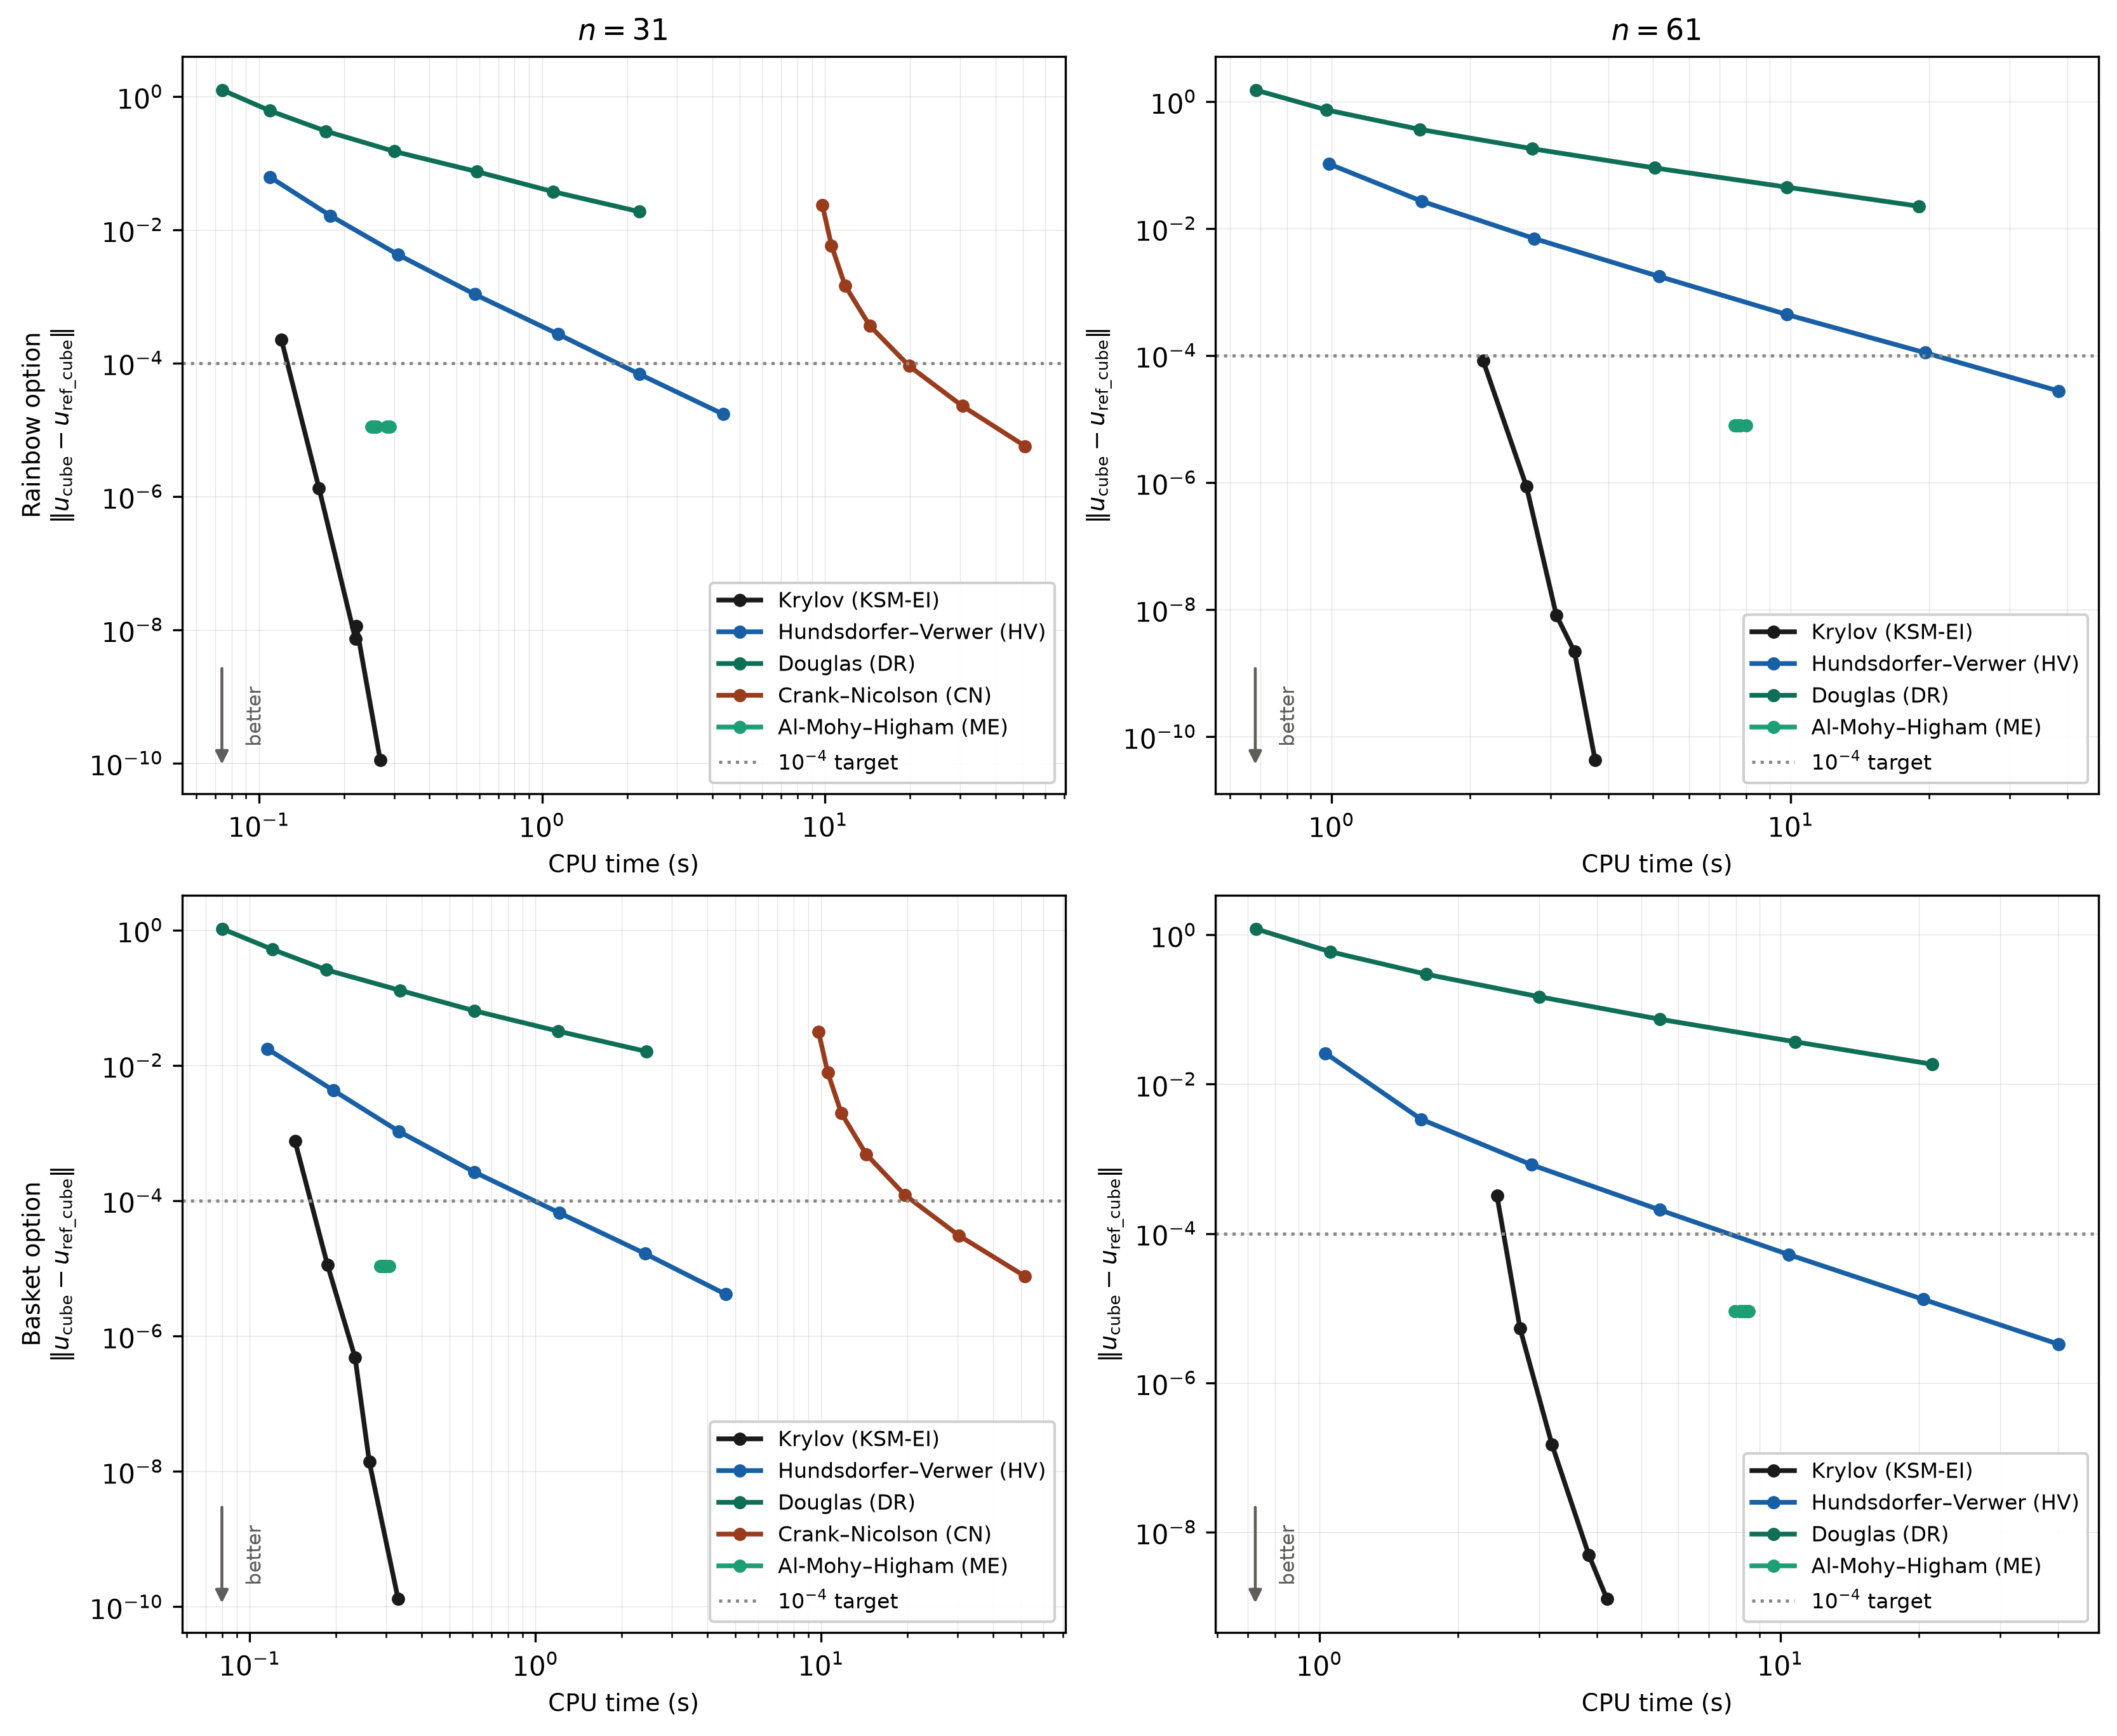
\includegraphics[width=0.62\textwidth]{benchmark_plots.png}
\caption{Semi-discrete ODE error vs.\ CPU time for the five methods, across both payoffs and grid sizes, following the historical Niesen--Wright option-pricing comparison. The Krylov integrator is fastest in the ${\sim}10^{-4}$ temporal-accuracy band for these runs; Crank--Nicolson's non-monotone stiff-mode ringing ($R(-\infty) = -1$) is visible.}
\label{fig:benchmark}
\end{figure}

\paragraph{The referee.} The reference is a high-accuracy solution of the same semi-discrete ODE, not an analytic or independent financial price. Before benchmarking each option type, the matrix-exponential referee uses maximum Taylor degree $m=55$ and $\theta=9.9$. The internal substep count is
\[
s=\left\lceil T\lVert\widetilde{\mat{A}}\rVert_1/\theta\right\rceil,
\]
at tolerance $2^{-53}\approx1.1\times10^{-16}$. The experiment isolates temporal-integration error. It does not include spatial discretization, finite-domain truncation, boundary-condition, or interpolation error, so it cannot establish total price or Greek accuracy.
The reported ODE error is the Euclidean norm over the $9\times9\times9$ grid neighborhood centered on the spot, not the value at one node. This avoids letting one fortuitously accurate node decide the comparison and samples the local surface used to extract price sensitivities.

\paragraph{Role of the benchmark.} The Niesen--Wright comparison serves as a historical control on the temporal integrators and their implementation. At $n=15$ every method reaches the same semi-discrete floor, so further temporal work buys nothing on that grid. The result motivates studying the Krylov implementation at larger states but does not establish contemporary pricing competitiveness. That claim would require equal-total-accuracy comparisons with alternatives such as the GPU ADI implementation of Dang, Christara, and Jackson for the same three-asset basket and rainbow contracts \cite{dang-christara-jackson-2010}. At larger asset counts, simulation methods with dimension reduction provide a more appropriate comparison because the full PDE grid grows exponentially with dimension \cite{wang-2009,weng-wang-he-2017}.
